%header and footer for separate chapter files

\ifx\whole\undefined
\documentclass[12pt, leqno]{book}
\usepackage{graphicx}
\input style-for-curves.sty
\usepackage{hyperref}
\usepackage{showkeys} %This shows the labels.
%\usepackage{SLAG,msribib,local}
%\usepackage{amsmath,amscd,amsthm,amssymb,amsxtra,latexsym,epsfig,epic,graphics}
%\usepackage[matrix,arrow,curve]{xy}
%\usepackage{graphicx}
%\usepackage{diagrams}
%
%%\usepackage{amsrefs}
%%%%%%%%%%%%%%%%%%%%%%%%%%%%%%%%%%%%%%%%%%
%%\textwidth16cm
%%\textheight20cm
%%\topmargin-2cm
%\oddsidemargin.8cm
%\evensidemargin1cm
%
%%%%%%Definitions
%\input preamble.tex
%\input style-for-curves.sty
%\def\TU{{\bf U}}
%\def\AA{{\mathbb A}}
%\def\BB{{\mathbb B}}
%\def\CC{{\mathbb C}}
%\def\QQ{{\mathbb Q}}
%\def\RR{{\mathbb R}}
%\def\facet{{\bf facet}}
%\def\image{{\rm image}}
%\def\cE{{\cal E}}
%\def\cF{{\cal F}}
%\def\cG{{\cal G}}
%\def\cH{{\cal H}}
%\def\cHom{{{\cal H}om}}
%\def\h{{\rm h}}
% \def\bs{{Boij-S\"oderberg{} }}
%
%\makeatletter
%\def\Ddots{\mathinner{\mkern1mu\raise\p@
%\vbox{\kern7\p@\hbox{.}}\mkern2mu
%\raise4\p@\hbox{.}\mkern2mu\raise7\p@\hbox{.}\mkern1mu}}
%\makeatother

%%
%\pagestyle{myheadings}

%\input style-for-curves.tex
%\documentclass{cambridge7A}
%\usepackage{hatcher_revised} 
%\usepackage{3264}
   
\errorcontextlines=1000
%\usepackage{makeidx}
\let\see\relax
\usepackage{makeidx}
\makeindex
% \index{word} in the doc; \index{variety!algebraic} gives variety, algebraic
% PUT a % after each \index{***}

\overfullrule=5pt
\catcode`\@\active
\def@{\mskip1.5mu} %produce a small space in math with an @

\title{Personalities of Curves}
\author{\copyright David Eisenbud and Joe Harris}
%%\includeonly{%
%0-intro,01-ChowRingDogma,02-FirstExamples,03-Grassmannians,04-GeneralGrassmannians
%,05-VectorBundlesAndChernClasses,06-LinesOnHypersurfaces,07-SingularElementsOfLinearSeries,
%08-ParameterSpaces,
%bib
%}

\date{\today}
%%\date{}
%\title{Curves}
%%{\normalsize ***Preliminary Version***}} 
%\author{David Eisenbud and Joe Harris }
%
%\begin{document}

\begin{document}
\maketitle

\pagenumbering{roman}
\setcounter{page}{5}
%\begin{5}
%\end{5}
\pagenumbering{arabic}
\tableofcontents
\fi


\chapter{The Riemann-Roch Theorem}

\subsection{Measuring linear series}

Because we are going to study curves via their maps to projective spaces, we will want to know how large a space of global
sections we should expect an invertible sheaf to have. We will answer this in several ways, but the beginning
of the story is the Riemann-Roch theorem.

We will henceforward assume that the reader is acquainted with sheaf cohomology, at least sufficiently to write
$H^i(X, \sF)$ without blushing. Note that if $\sF$ is a sheaf on $X$ and $X\subset Y$ then the cohomology  $H^i(X, \sF) = H^i(Y,\sF)$ canonically, so we will
simply and unambiguously write $H^i(\sF)$ for either of these. 
We write $h^i(\sF)$ or (if $D$ is a divisor) $h^{i}(D)$ for $\dim_{\CC}H^i(\sF)$ or $\dim_{\CC}H^i(D)$. 

Since we need lots of global sections of a line bundle $\sL$ to produce interesting maps from a curve $C$, we would like to be able to compute  $h^0(\sL) = \dim H^0(\sL)$. Much easier is to compute a sort of approximation to this number,
$$
\chi(\sL):= \sum_{i\geq 0} (-1)^i h^i(\sL),
$$
which makes sense, and even computes $h^0(\cL)$ itself in many cases, by virtue of the following result:

\begin{theorem} (Vanishing Theorem)
If $\sF$ is a coherent sheaf on a scheme $X$ of dimension $n$, then for any $i$, the vector space $H^i(\sF)$ is finite dimensional, and 0 if  $i>\dim X$. Moreover,
if $X\subset \PP^m$, then $H^i(\sF(d)) = 0$ for all $i>0$ and $d\gg 0$.\qed
\end{theorem}

\begin{proof}
This is a combination of Theorems \ref{Theorems III.2.7 and III.5.2}{H}, due to Grothendieck and Serre.
\end{proof}

Thus on a scheme $X\subset \PP^r$ we have $\chi(\sL(d) = h^0(\sL(d)$ for large $d$, and in the case of a curve $C\subset \PP^r$, we have $\chi(\sL = h^0(\sL) - h^1(\sL)$ as well.

\begin{theorem} (Easy Riemann-Roch)\label{easy RR}
If $C$ is a smooth curve, and $\sL$ is an invertible sheaf on $C$, then $\chi(\sL) = \deg \sL + \chi(\sO_C)$.
\end{theorem}

\begin{proof}
 The result is tautological if $\sL = \sO_C$. Every invertible sheaf on $C$ has the form $\sL = \sO_C(D)$ for some
divisor $D$. If $p\in C$, then writing $\kappa(p)$ for the 1-dimensional skyscraper sheaf at $p$, the long exact sequence in cohomology
associated to the short exact sequence
$$
0\to \sL(-p) \to \sL \to \sL\otimes \kappa(p)
$$
allows us to compute 
$$
\chi(\sL) = \chi(\sL(-p)) + \chi(\kappa(p)) = \chi(\sL(-p)) + 1.
$$
Since every divisor on $C$ can be reached by adding and subtracting points, this suffices.
\end{proof}

We can make a more useful Riemann-Roch theorem by understanding the error term $h^1(\sL)$ using
the canonical divisor and Serre duality, to which
we now turn.


\section{The most interesting linear series}

The most important vector bundles on a manifold are the tangent and cotangent bundles. For reasons that
will become clear, the focus in algebraic geometry is on the cotangent bundle or, equivalently, the sheaf of differential forms. On a smooth curve $C$, this is usually called the \emph{canonical sheaf} (on a smooth
variety of dimension $n$ the canonical sheaf is the $n$-exterior power of the sheaf of differentials). A section of 
$\omega_C$ is thus a differential form, and the class of the divisor
of such a form is usually denoted $K_X$. 

\begin{fact}
A famous result asserted by Franchetta and proved in~\cite{Harer} (see also~\cite{MR895568} and~\cite{MR1984659}) states that the canonical sheaf (and its powers) are the \emph{only} invertible sheaves that can be chosen uniformly on all, or even almost all, smooth curves. 
\end{fact}

On projective space we can compute the canonical sheaf directly; other computations of the canonical sheaf will usually reduce to this central case.

\begin{theorem}
 The canonical sheaf of $\PP^{r}$ is $\sO_{\PP^{r}}(-r-1)$. 
\end{theorem}
\begin{proof}
Let $x_{0}, \dots, x_{r}$ be the projective coordinates on $\PP^{r}$ and let  $U = \PP^{r}\setminus H$ be the affine open set where $x_{0} \neq 0$. Thus $U \cong \AA^{r}$ with coordinates $z_{1 := }x_{1}/x_{0}, \dots, z_{r}:=x_{r}/x_{0}$. The space of $r$-dimensional differential forms on $U$ is spanned by $d(x_{1}/x_{0})\wedge\cdots\wedge d(x_{r}/x_{0})$, which is regular everywhere in $U$. In view of the formula
$$
d\frac{x_{i}}{x_{0}} = \frac{x_{0}dx_{i}-x_{i}dx_{0}}{x_{0}^{2}}
$$
we get
$$
d(x_{1}/x_{0})\wedge\cdots\wedge d(x_{r}/x_{0}) = \frac{dx_{1}\wedge\cdots\wedge dx_{r}}{x_{0}^{r}}-
\sum_{i=1}^{r} x_{i} \frac{ dx_{1}\wedge\cdots \wedge \widehat{d_{x_{i}}}\wedge \cdots \wedge dx_{r}}{x_{0}^{r+1}}
$$
which has a pole of order $r+1$ along the locus $H$ defined by $x_{0}$. Thus the divisor of this differential form
is $-(r+1)H$, and this is the canonical class.
\end{proof}

\begin{fact}
A different derivation: there is a short exact sequence of sheaves, called the Euler sequence:
$$
0\to \Omega_{\PP^{r}} \to \sO_{\PP^{r}}^{r+1} (-1) \to \sO_{\PP^{r}} \to 0.
$$
Summing over all twists, and taking global sections, that is, applying $H^0_*$, we see that 
$H^0_*(\Omega_{\PP^{r}})$ fits into an exact sequence:
$$
0 \to H^0_*(\Omega_{\PP^{r}}) \rTo S^{r+1}(-1) \rTo^{\delta_{1}} S \rTo \CC \to 0,
$$
where $S$ is the homogeneous coordinate ring of $\PP^r$ and $\delta_1$ sends the $i$-th basis vector of
$S^{r+1}(-1)$ to the $i$-th variable of $S$; that is, $H^0_*(\Omega_{\PP^{r}})$ is the second syzygy of the residue field $\CC$ of $S$. We can extend this sequece to  the free resolution
of $\CC$, the Koszul complex:
$$
0 \to S(-r-1) \rTo^{\delta_{r+1}} \bigwedge^rS^{r+1}(-r) \rTo^{\delta_{r}} \cdots \rTo S^{r+1}(-1) \rTo S \to \CC \to 0.
$$
For each $i$, the $i$-th exterior power of the map $H^0_*(\Omega_{\PP^{r}}) \rTo S^{r+1}(-1)$ is an inclusion, and
represents $\bigwedge^i(\Omega_{\PP^{r}})$ as the sheaf associated to the graded module that is the $(i+1)$-st syzygy of $\CC$.
In particular, the canonical module $\omega_{\PP^r} = \bigwedge^r(\Omega_{\PP^{r}})$ is the sheaf associated to the 
$(r+1)$-st syzygy, $S(-r-1)$.
\end{fact}

The most important invariant of a smooth curve can be defined in terms of the canonical sheaf:

\begin{definition}
If $C$ is a smooth curve we define the genus $g(C)$ to be the dimension of $H^0(\omega_C)$.
\end{definition}

Computations of the canonical sheaf on a variety usually involve comparing the variety to a variety where the canonical sheaf is already known. The most useful results of this type are  the \emph{adjunction formula}
and \emph{Hurwitz' Theorem}. 

\subsection{The Adjunction Formula}\label{Adjunction Formula}

The adjunction formula describes the difference between the canonical divisor of
a codimension 1 subvariety and the restriction of the canonical divisor of the ambient variety.

\begin{proposition}\label{adjunction}(Adjunction Formula)
 Let $X$ be a variety that is a Cartier divisor on a variety $Y$, and let $K_{Y}$ be the canonical class of $Y$. The canonical class $K_X$ of $X$ is
 the restriction to $X$ of the divisor $K_{Y}+X$ on $Y$.
\end{proposition}
This is \cite[Proposition 8.20]{H}.
\begin{proof}
 There is an exact sequence of sheaves
 $$
0\to  \sI_{X/Y}\mid_{X} \to \Omega_{Y}\mid _{X} \to \Omega_{X} \to 0
 $$
 where $\Omega_{X}$ is the sheaf of differential forms on $X$ (see \cite[Proposition 16.3]{Eisenbud95}), and
$ \sI_{X/Y}\mid_{X} = \sO_{Y}(-X)\mid_{X} = \sO_{X}(-X)$. The proposition follows by taking top exterior powers.
\end{proof}

\begin{corollary}\label{canonical of plane curve}
If $C\subset \PP^{2}$ is a smooth plane curve of degree $d$, then $\omega_{C} = \sO_{C}(d-3)$; more generally, if
$X\subset \PP^{r}$ is a complete intersection of hypersurfaces of degrees $d_{1},\dots, d_{c}$ in $\PP^r$ then
$\omega_{X} = \sO_{X}(\sum_{i}d_{i }-r-1).$
\end{corollary}

\subsection{Hurwitz' Theorem}
 Given a (nonconstant) morphism $f : C \to X$ of smooth projective curves, the Riemann-Hurwitz formula computes the canonical sheaf  $C$ in terms of that of  $X$ and the local geometry of $f$. To do this we define the
\emph{ramification index} of $f$ at $p$,  denoted $\ram(f,p)$. In terms of a suitable choice of local coordinates $z$ on $C$ around $p$ and $w$ on $X$ around $f(p)$, we can write the morphism as $z \mapsto w = z^m$ for some integer $m > 0$, and $\ram(f,p) = m-1$. We could also define the ramification indices
by the formula of divisors
$$
 f^{-1}(f(q)) = \sum_{p\in C \mid f(p)=f(q)} (\ram(f,p)+1)\cdot p.
 $$
It follows from complex analysis (or the separability of field extensions in characteristic 0) that there are only finitely many
points on $C$ where $\ram(f,p) \neq 0$. Thus we can define the \emph{ramification divisor} of $f$ to be the divisor
 $$
 R = \sum_{p \in C} \ram(f,p)\cdot p \; \in \;  \Div(C).
 $$
 and the \emph{branch divisor} to be
 $$
 B = \sum_{q \in X} \Big(\sum_{p \in f^{-1}(q)} \ram(f,p) \Big)\cdot q \; \in \; \Div(X).
 $$
 Note that $R$ and $B$ have the same degree $\sum_{p \in C} \ram(f,p)$. 

 Hurwitz' theorem describes the difference between the canonical divisor of $C$ and the pullback of the canonical divisor of $X$.
\begin{theorem}(Hurwitz' Theorem) \cite[Proposition IV.2.3]{H} \label{Hurwitz}
If $f:C\to X$ is a non-constant morphism of smooth curves, with ramification divisor $R$, then 
$$
K_C = f^{*}(K_{X})+R,$$
or equivalently
$
\omega_{C} = (f^{*}\omega_{X})(R).
$
\end{theorem}
 
\begin{proof}
Choose a rational 1-form $\omega$ on $X$, and let $\eta = f^*(\omega)$ be its pullback to $C$. For simplicity, we will assume that the zeroes and poles of $\omega$ lie outside the branch divisor $B$, so that $\omega$ will be regular and nonzero at each branch point. (Since we have the freedom to multiply by any rational function on $X$ we can certainly find such a form, and in any event the calculation goes through without this assumption, albeit with more complicated notation.) 

Since the zeroes of $\omega$ lie outside the branch divisor $B$, for every zero of $\omega$ of multiplicity $m$ we have exactly $d$ zeroes of $\eta$, each with multiplicity $m$; and likewise for the poles of $\omega$. Meanwhile, at every point of $B$, the form $\omega$ is regular and nonzero. At a point $p$ where (locally) $f$ has the form $z \mapsto w = z^{e}$
and $\omega = dw,\ \eta dz$ we have $\eta = z^{e-1}dz$; that is $\eta$ has a zero of multiplicity $\ram(f,p)$ at  $p$.
Thus the divisor $K_{C}$ of $\eta$ is
$K_{C} = f^{*}(K_{X})+R$.
\end{proof}

\begin{example}
Let $C\subset \PP^2$ be a smooth plane curve and let $p\in \PP^2$ be a general point, with ideal
sheaf generated by the vector space of linear forms $W = \langle x_0,x_1\rangle$. 
The linear series $(\sO_C(1), W)$ defines the projection of $C$ from $p$ to $\PP^1$, a map of degree
$d = \deg C$.
\fix{insert picture}. The canonical sheaf of $\PP^1$ has degree $-2$, so by Hurwitz' theorem
$K_C$ has degree $ -2d+ \deg R$, where $R$ is the branch locus. We may choose coordinates
so that none of the branch points lie on the line $x_0 = 0$. Taking this to be the line at infinity, we
may compute the branch locus after passing to the affine open set $x_0\neq 0$, where the projection
map is given by the function $z = x_1/x_0$.  Suppose that $C$ is defined, in this open set,
by the equation $f(x,y)= 0$. A point $q\in C$ is a branch point if the tangent line to $C$ at $q$
passes through $p$, that is, if $dx$  and 
$$
df = \frac{\partial f}{\partial x} dx + \frac{\partial f}{\partial y} dy
$$
are linearly dependent, that is, if $\partial f/{\partial y}$ vanishes at $q$. The intersection of 
$C$ with the curve defined by $\partial f/{\partial y}=0$ has degree $d(d-1)$ by Bezout's theorem,
so the degree of the ramification divisor $R$ is $d(d-1)$ whence the degree of the canonical
divisor on $C$ is $\deg K_C = -2d+d(d-1) = d(d-3)$, which is in accord with 
Corollary~\ref{canonical of plane curve}.

\end{example}

\begin{example}
 Let $V$ be the vector space of homogeneous polynomials of degree $d$ in two variables; that is, $V = H^0(\cO_{\PP^1}(d))$. In the projectivization $\PP(V^{*}) \cong \PP^d$, let $\Delta$ be the locus of polynomials with a repeated factor. Since $\Delta$ is defined by the vanishing of the discriminant, it is a hypersurface. What is its degree?
 
 To answer this, let $W\subset V$ be a general 2-dimensional linear subspace---that is, a general pencil of forms of degree $d$ on $\PP^1$. The linear series $\sW = (\sO_{\PP^{1}}, W)$ defines a morphism $\phi_{\sW} : \PP^{1} \to \PP(W) \cong \PP^{1}$ and the fiber over the point of $\PP(W)$ corresponding to a form $f$ of degree $d$ is the divisor $\{f = 0\}\subset \PP^{1}$. Thus the locus of polynomials in $W$ with a multiple root is the branch locus of $\phi_{\sW}$, where we count an $m$-fold root $m-1$ times.
 By Hurwitz' formula, the degree of the branch locus $B$ of a degree $d$ morphism from $\PP^{1}$ to $\PP^{1}$ is
 $$
 \deg B = \deg \omega_{\PP^{1}} - d\deg \omega_{\PP^{1}} = 2d-2.
 $$
 \end{example}
  

\section{Genus, Riemann-Roch and Serre Duality}

We now return to the task of understanding $h^0(\sL)$ for an invertible sheaf $\sL$ on a smooth curve. Since $\chi(\sL) = h^0(\sL)-h^1(\sL)$ is easier to compute, we would like to understand $h^1(\sL)$ in a more concrete way. The key is duality:


%We will often wish to compute $h^0(\sL)$ for some
%sheaf $\sL$, and find that we can more easily compute 
%The (Zariski) Euler characteristic 
%$$
%\chi(\sL) = \sum_{i=0}^\infty (-1)^ih^i(\sL).
%$$
%
%Since $h^{i}(\sF)$ may be thought of in this way as an ``error term'' in formulas when one would like to compute
%$h^{0}(\sF)$,  vanishing theorems have an important place in all of algebraic and analytic geometry. We will use the simplest of these often:
%
%
%\begin{theorem}[Serre Vanishing Theorem]\label{Serre vanishing} If $\sF$ is a coherent sheaf on $\PP^n$, then
%$H^{i}(\sF)= 0$ for all $i>\dim \supp \sF$; and  $H^{i}(\sF(d))= 0$ for all $i>0$ and $d\gg 0$  
%\end{theorem}
%
%Using the second part of Theorem~\ref{Serre vanishing}, we see that the Euler characteristic of a coherent sheaf $\sF$ on a curve
% is  $\chi(\sF) = h^0(\sF) - h^1(\sF)$.
% 
% The other important cohomological result we will use is duality. We will use it only for invertible sheaves on curves, so we give it in
% that special case:
 
\begin{theorem}[Serre Duality]\label{sd}
If $C$ is a smooth curve and $D$ is a divisor on $C$, then
$$
H^1(D) =H^0(K_C-D)^*,
$$
and thus $h^1(D) = h^0(K_C-D)$.
\end{theorem}

For proofs see \cite[Theorem III.5.2 and III.7.6]{H}. 

For example we see that $h^1 (\sO_C) = h^0(K_C) = g(C)$.   
Using this we can recast the Easy Riemann-Roch theorem above in a more useful form. 

\begin{theorem} (Riemann-Roch)
If $C$ is a smooth curve, then $\chi(\sO_C) = 1-g(C)$.
If $D$ is any divisor on $C$, then 
$$
h^0(D) - h^0(K_C -D) = \deg D - g(C) +1.
$$
\end{theorem}

\begin{proof}
Combine Theorem~\ref{easy RR} with Theorem~\ref{sd}.
\end{proof}
Applying the formula with $D = K_C$, we get 
$\deg K_C = 2g(C) -2$.

We can now explain the relationship between the genus of a smooth curve, as we have defined it and the 
topological genus, the ``number of holes'' in the Riemann surface:
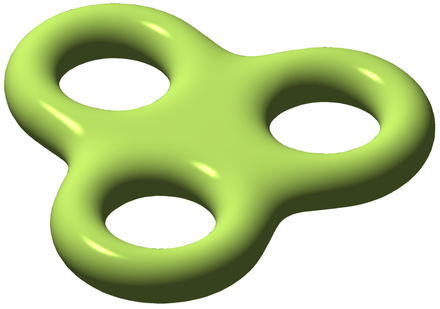
\includegraphics[scale = 1]{RiemannSurface}
**** Riemann Surface of genus 3, from Wikimedia ****

\begin{fact} (Hodge Theory)
The sole topological invariant of a smooth projective curve $C$ is its genus. As a manifold it is a compact, oriented surface, and its genus is half the rank of its first singular cohomology, $H^{1}(C; \CC)$, which is equal to its first deRham cohomology.
Breaking up the deRham cohomology of any smooth complex variety $X$ in terms of holomorphic and antiholomorphic differential
forms we get the \emph{Hodge decomposition}
$$
H^i(X,\CC) = H^i_{\rm de Rham}(X) = \bigoplus_{j=0}^i H^j(\bigwedge^{i-j} \Omega_X).
$$
For a smooth curve $C$, this says in  particular that
$$
H^1(C; \CC) = H^0(\omega_C)\oplus H^1(\sO_C) = H^0(\omega_C)\oplus (H^0(\omega_C))^\vee, 
$$
so $ h^0(\omega_C)$ is half the rank of the middle singular cohomology group, justifying the name ``genus''.
\end{fact}


If $E$ is a divisor of negative degree then $H^0(E) = 0$ so we get the form of the Riemann-Roch theorem
originally proved by Riemann:

\begin{corollary}\label{nonspecial RR}
For any divisor $D$ of degree $d$ we have
$$
h^0(D) \geq d - g + 1,
$$
with equality if $d > 2g-2$.
\end{corollary}
It was Riemann's student Roch  who supplied the correction term $h^0(K_C - D)$ for divisors of lower degree.
The dimension $h^0(K_C-D) = h^1(D)$ was called the \emph{superabundance} of $D$.

Corollary~\ref{nonspecial RR} and Proposition~\ref{very ample} together show that all high degree divisors come from hyperplane sections in 
suitable embeddings:

\begin{corollary}\label{degree 2g+1 embedding}
Let $D$ be a divisor of degree $d$ on a smooth, connected projective curve of genus $g$. If $d \geq 2g$, the complete linear series $|D|$ is base point free; and if $d \geq 2g+1$ the associated morphism $\phi_D : C \to \PP^{d-g}$ is an embedding, so that
$D$ is the preimage of the intersection of $C$ with a hyperplane in $ \PP^{d-g}$.
\end{corollary}

Since the complement of a hyperplane in projective space is an affine space, we get an affine embedding result too:

\begin{corollary}
 If $C$ is any smooth, connected projective curve and $\emptyset \neq \Gamma \subset C$ a finite subset then $C \setminus \Gamma$ is affine.
\end{corollary}
\begin{proof}
Let $D$ be the divisor defined by $\Gamma$. By Corollary~\ref{degree 2g+1 embedding} a high multiple of $D$ is very ample,
and gives an embedding $\phi: C\to \PP^n$ such that the preimage of the intersection of $C$ with some hyperplane $H$
is a multiple of $D$. It follows that $C\setminus \Gamma$ is embedded in $\AA^n = \PP^n\setminus H$.
\end{proof}
 
We can  use Corollary~\ref{nonspecial RR} to determine the Hilbert polynomial of a projective curve. To do this, let $C \subset \PP^r$ be a smooth curve of degree $d$ and genus $g$, and consider the exact sequence of sheaves
$$
0 \rTo \cI_{C/\PP^r}(m) \rTo \cO_{\PP^r}(m) \rTo \cO_C(m) \rTo 0
$$
and the corresponding exact sequence
$$
 H^0(\cO_{\PP^r}(m)) \rTo^{\rho_m} H^0(\cO_C(m)) \rTo H^1(\cI_{C/\PP^r}(m)) \rTo 0.
$$

The \emph{Hilbert function} $h_C$ of $C$  is defined by
$$
h_C(m) = \dim_{\CC} (S_{C})_{m} = \rank(\rho_m).
$$
By Theorem~\ref{Serre vanishing} we have $H^1(\cI_{C/\PP^r}(m)) = 0$ for large $m$, so $h_{C}(m) = h^0(\cO_C(m))$ for large $m$, which, by the Riemann-Roch theorem, equals $md-g+1$, again for large $m$. Thus, the Hilbert polynomial of $C \subset \PP^r$ is $p_C(m) = dm-g+1$, establishing the characterization~(\ref{genus Hilbert}).
 
The Riemann-Roch formula does \emph{not} give us a formula for the dimension $h^0(D)$ when $h^0(K_C - D)>0$; such divisors $D$ are called \emph{special divisors}. The existence or non-existence of divisors $D$ with given $h^{0}(D)$ and $h^{1}(D)$ often serves to distinguish one curve from another, and will be an important part of our study.


%\subsection{Proof of Theorem~\ref{RR} from Theorem~\ref{sd}.}
%
%If, following~\ref[Chapter IV]{H} we take the definition of the genus of  a smooth connected curve $C$ to be $h^1(\sO_C)$ (so that $g = h^0(K_C)$ becomes a Corollary of Theorem~\ref{sd}), then it is easy to establish the following form of the Riemann-Roch Theorem:
%
%\begin{corollary}
% If $C$ is a smooth, connected projective curve and $D$ is a divisor on $C$ then
%$$
%\chi(\sO_C(C)) := h^0(D) - h^1(D) = d-g+1
%$$
%or in other words, for any invertible sheaf $\cL$ of degree $d$ on $C$,
%$$
%\chi(\cL) = d-g+1.
%$$
%\end{corollary}
%\begin{proof}
% Taking $D=0$ the statement becomes $h^0(\sO) - h^1(\sO) = 1-g$, which is our definition of $g$. On the other hand,
%for any divisor $D$ on $C$ and any point $p \in C$ we have an exact sequence of sheaves
%$$
%0 \to \cO_C(D-p) \to \cO_C(D) \to \frac{\cO_C(D)}{\gm_{C,p}\cO_C(D)} \to 0
%$$
%Since $\cO_C(D)$ is locally isomorphic to $\sO_C$ we see that $\cO_C(D)/\gm_{C,p}\cO_C(D)\cong \kappa(p)$ is a sky-scraper sheaf of dimension 1, concentrated at $p$,
%and thus has Euler characteristic 1. 
%
%Thus the Riemann-Roch Theorem for $\cO_C(D)$ is equivalent to the Riemann-Roch Theorem for $\cO_C(D-p)$. Since any divisor can be obtained from 0 by adding and subtracting points, the Riemann-Roch formula for an arbitrary $\cL$ follows from the special case $\cL = \cO_C$ with which we began.
%\end{proof}


\subsection{Arithmetic genus and geometric genus}
In this section, we'll deal with a  curve $C_0$ that is assumed to be reduced and irreducible, but not necessarily smooth.
Given $C_0$ there is a unique normalization morphism $\nu: C \to C_0$, and thus $C_0$ is birational to a unique
smooth curve. The genus of $C$ is called the \emph{geometric genus} of $C_0$.

Most of the results of this book have analogues for singular curves, but this is a topic beyond our scope; for us, the questions are about smooth curves, with singular curves appearing as a useful adjunct, for example in Chapter~\ref{PlaneCurveChapter}.

Applied to a possibly singular or even non-reduced 1-dimensional projective scheme, the formula~\ref{pa} and the equivalent~\ref{genus Hilbert}, define
what is called the \emph{arithmetic genus} $p_a(C)$. 

We can relate the arithmetic and geometric genera of $C_0$ using the map of sheaves
$$
\cO_{C_0} \to \nu_*\cO_C.
$$
This is injective; the cokernel sheaf will be a skyscraper sheaf supported on the singular points of $C_0$. Denoting this sheaf by $\cF$, we have an exact sequence
$$
0 \to \cO_{C_0} \to \nu_*\cO_C \to \cF \to 0.
$$


The normalization map $\nu: C \to C_0$ is finite, so that the direct images $R^i\nu_*\cO_C$ vanish for $i > 0$; it follows from the Leray spectral sequence~\ref{Leray} that $\chi(\nu_*\cO_C) = \chi(\cO_C)$. Thus
$$
p_a(C_0) - g(C) =  \chi(\cO_{C}) -   \chi(\cO_{C_0}) = \chi(\cF) = h^0(\cF);
$$ 
in other words, the difference between the arithmetic and geometric genera of $C_0$ is the sum of the vector space dimensions of the stalks of $\cF$; colloquially, it's the number of linear conditions a function $f$ on $C$ has to satisfy to be the pullback of a function from $C_0$. The length of the stalk of $\cF$ at a particular singular point $p \in C_0$ is called the \emph{$\delta$-invariant} $\delta_p$ of the singularity; to rephrase the statement above in these terms, we have:
$$
p_a(C_0) - g(C) = \sum_{p \in (C_0)_{sing}} \delta_p
$$ 

\begin{fact}\label{Leray}
 We have used an almost trivial part of the Leray spectral sequence, and we shall use it again in a few other almost equally simple cases. Suppose that $f:X\to Y$ is a morphism of varieties or schemes
 and $\sF$ is a coherent sheaf on $X$.
  It follows immediately from the definition of the push-forward that $\HH^0(\sF) \cong \HH^0(f_*(\sF))$. Replacing
  $\sF$ by an injective or flasque resolution, we get the Leray spectral sequence
  $$
  \HH^p(R^qf_*(\sF)) \Longrightarrow \HH^{p+q}(\sF).
  $$
 \end{fact}
  


The $\delta$ invariant is easy to compute in simple cases:
\begin{enumerate}

\item (nodes) If $p \in C_0$ is a node, with points $r,s \in C$ lying over it, the condition for a function $f$ on $C$ to descend is simply that $f(r)=f(s)$; this is one linear condition so $\delta_p = 1$.

\item (cusps) If $p \in C_0$ is a cusp, with  $r \in C$ lying over it, the condition for a function $f$ on $C$ to descend is simply that the derivative $f'(r)=0$; again, this is one linear condition so $\delta_p = 1$.

\item (tacnodes) Suppose now that $p \in C_0$ is a \emph{tacnode}, that is, $C_0$ has two smooth branches at $p$ simply tangent to one another. There will be two points $r, s \in C$ lying over it, and the condition for a function $f$ on $C$ to descend is that in terms of suitable local coordinates both $f(r)=f(s)$ and $f'(r)=f'(s)$.  This represents two linear conditions, so $\delta_p = 2$.

\item (planar triple points) An ordinary triple point $p \in C_0$ of a plane curve is a singularity consisting of three smooth branches meeting pairwise transversely, such as the zero locus of $y^3-x^3$. There will be three points $r,s,t \in C$ lying over $p$, and certainly a necessary condition for a function $f$ on $C$ to descend is that $f(r)=f(s)=f(t)$---two linear conditions. But there's a third, less obvious linear condition: in order for $f$ to descend, the derivatives $f'(r), f'(s), f'(t)$ have to satisfy a linear condition---a reflection of the fact that a function on $C_0$ cannot vanish to order 2 on each of two branches without vanishing to order 2 along the third as well. Thus $\delta_p = 3$

\item (spatial triple points) We will be concerned in what follows only with planar singularities, but spatial triple points provide a useful contrast to the last example. A spatial triple point is a singularity consisting of three smooth branches, with linearly independent tangent lines, so that its Zariski tangent space is 3-dimensional. An example would be the union of the three coordinate axes in $\AA^3$.

In this case, in contrast to case of the planar triple point, the condition that $f(r)=f(s)=f(t)$ is both necessary and sufficient for $f$ to descend, and thus  $\delta_p=2$.

\end{enumerate}




\section{The canonical morphism}

We will generally begin to study the invertible sheaves on a smooth curve $C$ by studying the complete linear series associated to the canonical divisor $|K|$ and the \emph{canonical map}
 $\phi_K : C \to \PP^{g-1}$. 
 
 In the case $g=0$ the canonical sheaf has degree 0 and since it has nonzero global sections, 
 $\omega_C = \sO_C$, and $K_C = 0$. Thus we restrict our attention to smooth curves $C$ of genus $g\geq 2$. We will see
 that the canonical series is then base-point free, so $|K|$ defines a morphism.

Recall that a curve of genus $\geq 2$
is said to be \emph{hyperelliptic} if there exists a morphism $f: C \to \PP^1$ of degree 2. 


\begin{theorem}\label{canonical series is very ample}
If $C$ is a smooth curve of genus $\geq 2$ then the canonical morphism $\phi_K : C \to \PP^{g-1}$ is an embedding if and only if $C$ is not hyperelliptic. 
\end{theorem}

The image of the canonical morphism of a non-hyperelliptic curve of genus $g>2$ is called a \emph{canonical curve}.

\begin{proof}
By Corollary~\ref{degree 2g+1 embedding} we have to show that for any pair of points $p, q \in C$ we have
$$
h^0(K_C(-p-q)) = h^0(K_C)-2 = g-2.
$$
Applying \trr we see this fails if and only if $h^0(\cO_C(p+q)) \geq 2$ for some $p,q \in C$. By Lemma~\ref{deg 2 morphism}, this implies that $C$ is hyperelliptic.
\end{proof}

\begin{lemma}\label{deg 2 morphism}
Let $C$ be a smooth, projective curve of genus $g\geq 2$. If $C$ has an invertible sheaf $\cL$ of degree 2 with two independent sections, then
$|\cL|$ defines a morphism of degree 2 to $\PP^{1}$, and $C$ is hyperelliptic. In particular, if $g(C) = 2$ then the canonical series $|K_{C}|$ defines a 2 to 1 morphism to $\PP^{1}$, so $C$ is hyperelliptic.
\end{lemma}

\begin{proof}
If $\cO_C(p+q)$ has two independent sections and has $d$ basepoints, then it defines a morphism of degree $2-d$ to $\PP^1$. Since $C$ is not rational,
we must have $d=0$, proving the first statement. 
\end{proof}

\subsection{The geometric Riemann-Roch theorem}

If $C$ is a nonhyperelliptic curve, embedded in $\PP^{g-1}$ by its canonical series and  $D = p_1+\dots + p_d$ is a divisor consisting of $d$ distinct points, we will write $\overline D$ be the span of the points $p_i \in C \subset \PP^{g-1}$. Since the hyperplanes in $\PP^{g-1}$ containing $\{p_1,\dots,p_d\}$ correspond (up to scalars) to sections of $K_C$ vanishing at all the points $p_i$, we see that
$$
h^0(K_C-D) = g - 1 - \dim \overline D = \codim \overline D \subset \PP^{g-1}
$$
Plugging this into the Riemann-Roch formula, we arrive at the statement
$$
r(D) = d - 1 - \dim \overline D;
$$
or in other words, the dimension of the linear series $|D|$ in which the divisor $D$ moves is equal to the number of linear relations on the points $p_i$ on the canonical curve. Thus, for example, if $D = p_1+p_2+p_3$, we see that $D$ moves in a pencil if and only if the points $p_i$ become collinear under the canonical morphism.

We can extend this statement to the case of arbitrary effective divisors $D$ on any smooth curve if we define our terms correctly. To do this, suppose $f : C \to \PP^d$ is any morphism, and $D \subset C$ any divisor. We define the \emph{span} of  $f(D)$ to be the intersection
$$
\overline{f(D)} = \bigcap_{H \mid f^{-1}(H)\supset D} H 
$$
of all hyperplanes in $\PP^d$ whose preimage in $C$ contains $D$. The argument above applies to prove:

\begin{theorem}[Geometric Riemann-Roch Theorem]\label{geometric RR}
If $C$ is any curve of genus $g \geq 2$,  $\phi : C \to \PP^{g-1}$ its canonical morphism and $D \subset C$ any effective divisor of degree $d$, then
$$
r(D) = d - 1 - \dim \overline{\phi(D)}.
$$
\end{theorem}

\section{Clifford's theorem}

While the Riemann-Roch Theorem gives a lower bound for the dimension of a linear series, $r(\sL) := h^0(\sL)-1 \geq \deg \sL -g$, Clifford's Theorem
gives an upper bound. If $\deg \sL>2g-2$, then the Riemann-Roch inequality becomes an equality, so it is enough to treat the case $\deg \sL \leq 2g-2$. The bound is actually a corollary of the Riemann-Roch theorem 

\begin{corollary}\label{Clifford bound}
 Let $C$ be a curve of genus $g$ and $\cL$ a line bundle of degree $d \leq 2g-2$. Then
$$
r(\cL) \leq \frac{d}{2}.
$$
\end{corollary}

\begin{proof}
If $\cL$ is nonspecial then, since $g=geq d/2 + 1$, we have $r(\cL) = d-g+1\leq d/2$.
Otherwise we have
$$
r(K_C\otimes \cL^{-1}) = r(\cL) +g - d - 1
$$
by the Riemann-Roch Theorem,
and so by Proposition~\ref{sum of linear series}
$$
g-1 = r(K_C)  \geq r(\cL) + r(K_C\otimes \cL^{-1})  \geq 2r(\cL) +g - d-1;
$$
hence $r(\cL) \leq d/2$.
\end{proof}

The usual statement of Clifford's theorem includes a description of when equality can occur:
To state it, we define a curve $C$ of genus $\geq 2$ to be \emph{hyperelliptic} if there exists a $g^1_2$ on $C$: that is an
invertible sheaf $\cL$ of degree $2$ with 2 independent global sections or, equivalently, a morphism $C\to \PP^1$ of degree 2. We will see in Chapter~\ref{genus 2 and 3 chapter} that such a sheaf would be unique, and $h^0(\cL) = 2$, and that such curves have extremely special properties.

\begin{theorem}\label{Clifford}\label{Clifford equality}
Let $C$ be a curve of genus $g$ and $\cL$ a line bundle of degree $d \leq 2g-2$. If
$$
r(\cL) = \frac{d}{2},
$$
the largest possible value, then either
\begin{enumerate}
\item $d=0$ and $\cL = \cO_C$;
\item $d = 2g-2$ and $\cL = K_C$; or
\item $C$ is hyperelliptic, and $|\cL|$ is a multiple of the $g^1_2$ on $C$.
\end{enumerate}
\end{theorem}

For the proof of the second half of Clifford's Theorem, we will use a basic fact about the geometry of hyperplane sections of a curve in projective space (Proposition~\ref{monodromy of hyperplane section}); we give the proof after proving that result.


 \section{Curves on surfaces}
 We will often analyze curves  on a smooth surface. Compared to the theory of linear series on curves, there is a new element: the intersection pairing. We refer to~\cite[Chapter V]{Hartshorne1977}
 and~\cite[Chapter I]{Beauville} for proof of the unproven statements in this section.
 
 We suppose for this section that $X$ is a smooth projective surface.
 We define $\Pic(X)$ to be the group whose elements are invertible sheaves on $X$.
When two divisors $D,E$ on $X$ meet transversely we define $D\cdot E$ to be the number of points in which they meet. If they have no common
components, we can still define a non-negative intersection multiplicity $m_X(D,E,p)$ at each point $p$, and then set
$$
D\cdot E = \sum_p m_X(D,E,p).
$$
Over the complex numbers each codimension 1 subvariety $D$ of $X$ has a fundamental class
$[D]\in H^2(X, \ZZ)$ and the product is the cup product with values in $H^4(X,\ZZ)$, which is $\ZZ$ since $X$ is compact and orientable. Thus
there is an extension of the product to the cases where $D,E$ have common components. From a geometric point of view, we may choose an
appropriate $C^\infty$
normal vector field along $E$ and define $E'$ by ``pushing'' $E$ out slightly along the direction of this field, until $D$ and $E'$ are transverse,
and the intersections can be computed in the usual way. It should be noted that such intersection numbers can be either positive or negative,
since they depend on the relative orientations of $D$ and $E'$ at the intersection points; this is in contrast to the case when $D$ and $E$
themselves meet properly; in this case the fact that the complex numbers are canonically oriented makes the intersection number non-negative.

The intersection product can also be defined algebraically, over any field: Setting $\sL := \sO_X(C)$ and
$\sM := \sO_X(D)$ to simplify the notation, we set 
$$
D\cdot E = \chi(\sO_X)-\chi(\sL^{-1}) -\chi(\sM^{-1}) -\chi(\sL^{-1}\sM^{-1}) 
$$
\begin{theorem} The pairing $(D,E) \mapsto (D.E)$ is the unique bilinear map
$\Pic(X) \times \Pic(X) \to \ZZ$ extending the case of intersections of two transverse curves on $X$. 
\end{theorem}

A frequent use of the the intersection pairing is to compute the (arithmetic) genus of a curve on a surface,
a result called the adjunction formula.

\begin{theorem}[Adjunction Formula]\label{adjunction formula}
If $C$ is a curve lying on a smooth surface $X$ then 
$$
\omega_C = \omega_X \otimes \sO_X(C) \otimes \sO_C.
$$
In particular \label{genus formula}
$$
p_a(C) = \frac{(K_X+C)\cdot C}{2} +1
 $$
\end{theorem}

We will frequently be interested in curves on quadrics in $\PP^3$, and we can spell out the
intersection theory on these surfaces very concretely; see for example~\cite[Section V.1]{H}.
We will treat them and the curves on them in detail in Section~\ref{curves on scrolls} as part of the larger family of 2-dimensional rational normal scrolls; for
now we sketch the situation as an example of the theory of this section. 

\begin{example}[Quadrics in $\PP^3$]\label{Div of quadric}
 
Quadric surfaces $S$ in $\PP^3$ are classified by their rank:
\begin{itemize}
\item A quadric of rank 2 is the union of two planes; it cannot contain an nondegenerate irreducible curve
\item A rank 3 quadric $S$ is a cone over a plane conic. Suppose that $C$ is a smooth,
curve on such a quadric:
\begin{itemize}
\item  If $C$  does
not pass through the vertex then it is the intersection of the quadric with a hypersurface of some
degree $d$. In this case $C$ has degree $2d$ and genus $(d-1)^2$. 
 \item if $C$ passes through the vertex, then $C$ lies in the divisor class of a line through the origin plus the intersection of $S$ with a hypersurface of some degree $d$. In this case $C$ has degree $2d+1$ and 
 genus $d(d-1)$. 
\end{itemize}

%If  it contains smooth irreducible curves that do not pass through the vertex of the cone, and smooth irreducible curves that of
%degree $2d$ that are intersections of $S$ with hypersurfaces of degree $d$; and smooth 
%irreducible curves of degree $2d+1$ that 

\item A quadric of rank 4 is nonsingular, and is isomorphic to $\PP^1\times \PP^1$.


\item The Picard group of $\PP^1\times \PP^1$ is $\ZZ\oplus \ZZ$, generated by the 
classes of the lines $\{p\}\times \PP^1$ and $\PP^1\times \{p\}$, where $p\in \PP^1$
is any point. These lines have self-intersection 0, and meet transversely in a point,
so the intersection pairing is given by $(a,b)\cdot(c,d) = ad+bc$. From the adjunction formula
applied to the classes of the lines $(1,0)$ and $(0,1)$ we that the canonical
class is $(-2,-2)$, and thus the arithmetic genus of a curve of type $(a,b)$ is thus
$$
\left(((a,b)+(-2,-2))\cdot (a,b)\right)/2 +1 = (a-1)(b-1).
$$

\item Writing $\pi_1, \pi_2$ for the two projections of
$\PP^1\times \PP^1 \to \PP^1$, the sheaf 
$$
\sL := \sO_{\PP^1\times \PP^1}(a,b) = \pi_1^*\op1a \otimes \pi_2^*\op1b
$$
has cohomology given by the K\"unneth formula, for example
\begin{align*}
 H^0(\sL) &= H^0(\op1a)\otimes H^0(\op1b) \hbox{ and thus }\\
 h^0(\sL) &= (a+1)(b+1) \hbox{ if } a\geq 0, b\geq 0.
\end{align*}

\item Any smooth quadric surface $S\subset \PP^3$ is the 
image of $\PP^1\times \PP^1$ embedded by the complete linear series
$|\sO_{\PP^1\times \PP^1}(1,1)|$ and thus contains two families of lines. 
A curve in the class $(a,b)$ thus has degree $(a,b)\cdot(1,1) = a+b$. 
\end{itemize}
\end{example}

Often we wish to compute the dimension of the space of sections of an invertible sheaf, but
as with the case of curves, the Euler characteristic is more accessible:

\begin{theorem}[Riemann-Roch for surfaces] Let $\sL$ be an invertible sheaf on a smooth surface $S$.
the Euler characteristic $\chi(D) := h^0(\sL)-h^1(\sL)+h^2(\sL)$, where $\sL = \sO_S(D)$, is given by
$$
\chi(D) = \chi(\sO) + \frac{(D-K_S)\cdot D}{2}+1
$$
\end{theorem}

%\fix{Possible addition:  the Hodge Index theorem as corollary. This could be used to prove finiteness of the automorphism group of a curve following Hartshorne V Ex. 1.11, perhaps in place of the proof now in the inflections chapter.}

It is useful to know what happens under mappings of surfaces, particularly the case of the mapping
corresponding to blowing up a point.

\begin{theorem}
If $\pi: X \to Y$ is a birational map of smooth surfaces, then the pullback map on divisors
preserves the intersection pairing. If $X$ is the blowup of $Y$ at a point $p$, with exceptional
divisor $E = \pi^{-1}(p)$ then:

\begin{enumerate}
 \item $\Pic X =\pi^*(\Pic Y) \oplus \ZZ E$.
\item The canonical class on $X$ is given by $K_X = \pi^*(K_Y)+E$.
 \item The intersection pairing on $\Pic X$ is given by
 
\begin{itemize}
\item $\pi^*(D)\cdot\pi^*(D') = D.D'$ for all $D,D'\in \Pic Y$.
\item $\pi^*(D)\cdot E = 0$ for all $D\in \Pic Y$.
 \item $E\cdot E = -1$.
 \item $K_X\cdot E = -1$.
 \item If $C$ is a curve that has an $m$-fold point at $p$ then $\pi^{-1}(C)$ contains $E$ with multiplicity $m$.
 \end{itemize}
\end{enumerate}
\end{theorem}

Blowups occur frequently in the theory of surfaces, and are easy to characterize:
\begin{theorem}
If $E\subset X$ is a curve on a smooth projective surface $X$ and
 that $E^2 = E\cdot K_X = -1$ then $E$ can be ``blown down'' in the sense that
 $X$ is the blowup of a smooth surface $Y$ at a point $p\in Y$, and $E$ is the exceptional divisor.
\end{theorem}


\section{Exercises}

In the following series of exercises, we are going to be working with smooth projective curves associated to a given affine curve $C^\circ := V(f(x,y)) \subset \AA^2$; this is the unique smooth projective curve containing the normalization of $C^\circ$ as a Zariski dense open subset.

\begin{exercise}
Let $C$ be the smooth projective curve associated to the affine plane curve $y^3 +x^3 = 1$, and let $\pi : C \to \PP^1$ be the map given by the rational function $x$.
\begin{enumerate}
\item Find the branch points and ramification points of $\pi$, and deduce that the genus of $C$ is 1.
\item For any two points $p, q \in C$ find the complete linear series $|p+q|$.
\item Find the (unique) map $\eta : C \to \PP^1$ of degree 2 such that $\eta((1,0)) = \eta((0,1))$, and determine the ramification points of $\eta$.
\item Show that $C$ is isomorphic to the smooth projective curve associated to the affine plane curve $y^2 +x^3 = 1$.
\end{enumerate}
\end{exercise}

For the next three exercises, let $C^\circ$ be the affine plane curve given as the zero locus of $y^2 - x^6 +1$, and let $C$ be the corresponding smooth projective curve. Note that the map $C^\circ \to \AA^1$ given by the projection $(x,y) \mapsto x$ extends to a map $\pi : C \to \PP^1$, expressing $C$ as a 2-sheeted cover of $\PP^1$ branched over the points $1, \zeta, \dots, \zeta^5$, where $\zeta$ is any primitive 6th root of unity. In addition, let $p$ and $q \in C$ be the two points lying over the point $\infty \in \PP^1$.

\begin{exercise}\label{hyperelliptic curve 1}
Let $C^\circ$ be the affine plane curve given as the zero locus of $y^2 - x^6 +1$, and let $C$ be the corresponding smooth projective curve. 

Show  that the map $C^\circ \to \AA^1$ given by the projection $(x,y) \mapsto x$ extends to a map $\pi : C \to \PP^1$, expressing $C$ as a 2-sheeted cover of $\PP^1$ branched over the points $1, \zeta, \dots, \zeta^5$, where $\zeta$ is any primitive 6th root of unity. Show that there are two distinct points $p$ and $q \in C$  lying over the point $\infty \in \PP^1$,
so that $C$ is unramified over $\infty$.

What is the genus of $C$?
\end{exercise}

\begin{exercise} With $C$ as in Exercise~\ref{hyperelliptic curve 1}:
\begin{enumerate}

\item Let $r_\alpha$ be the branch point over $\zeta^\alpha$. Show that
$$
p+q \sim 2r_\alpha \quad \text{and} \quad \sum_{\alpha = 0}^5 r_\alpha \sim 3p+3q.
$$

\item Find the vector space $H^0(\cO_C(D))$ where $D = r_0 + r_2 + r_4$, and find the (unique) divisor $E$ on $C$ such that $E + r_1 \sim r_0 + r_2 + r_4$.

\end{enumerate}

\end{exercise}


\begin{exercise}
With $C$ as in Exercise~\ref{hyperelliptic curve 1}:
Let $D$ be the divisor $D = p + q + r_0 + r_3$
\begin{enumerate}
\item Find the vector space $H^0(\cO_C(D))$.
\item Describe the map $\phi_{|D|} : C \to \PP^2$.
\item Find the equation of the image curve $\phi_{|D|}(C) \subset \PP^2$, and describe its singularities.
\end{enumerate}
\end{exercise}

The following exercises deal with the curve 
\begin{exercise}
Let $C$ be the smooth projective curve associated to the affine curve $y^3 = x^5 -1$. Note that the map $\pi : C \to \PP^1$ given by the function $x$ expresses $C$ as a cyclic, 3-sheeted cover of $\PP^1$, branched over the 5th roots of unity and the point at $\infty$. By way of notation, if we take $\eta = e^{2\pi i/5}$ a primitive 5th root of unity, we'll denote by $r_\alpha$ the point $(\eta^\alpha, 0) \in C$ lying over $\eta^\alpha$, and by $p$ the point lying over $\infty \in \PP^1$.

\begin{enumerate}
\item Verify that there is indeed a unique point $p \in C$ lying over $\infty \in \PP^1$, and the map has ramification index 2 at $p$. 
\item Show that the genus of $C$ is 4.
\item Establish the linear equivalences
$$
3p \sim 3r_\alpha \quad \text{and} \quad r_1+ \dots + r_5 \sim 5p.
$$
\item Find a basis for the space $H^0(K_C)$ of regular differentials on $C$.
\item Show that $C$ is not hyperelliptic.
\item Describe the canonical map $\phi_K : C \to \PP^3$ and find the equations of the image.
\item Let $D$ be the divisor $D = r_1+\dots+r_5$. Show that $h^0(K_C(-D)) = 1$; deduce that $r(D) = 2$, and find a basis for $H^0(\cO_C(D))$.
\item If $E = 3p$, show that $r(E) = 1$; that $|E|$ is the unique $g^1_3$ on $C$ and that $2E \sim K$.
\end{enumerate}
\end{exercise}


\begin{exercise}\label{gonality exclusion}
Show that a curve of genus $g \geq 3$ cannot be simultaneously hyperelliptic and a three-sheeted cover of $\PP^1$.
\end{exercise}

\begin{exercise}
Show that normalization of the affine planar triple point $xy(x-y) = 0$ in $\AA^2$ is the disjoint union of three
affine lines, $\Spec(\CC[x] \times \CC[y]\times \CC[z]$. Compute the linear conditions on the values and derivatives of three polynomial functions f,g,h defined on
these three lines that they ``descend'' to give a well-defined function on the planar triple point.
\end{exercise}

\begin{exercise} Generalize the results on planar triple points, above, to the case of a plane curve with $n$ pairwise
transverse branches, called an \emph{ordinary multiple point}.
\end{exercise}

\begin{exercise}
Let $p \in C$ be a singular point of a reduced curve $C$. Show that if $\delta_p = 1$, then $p$ must be either a node or a cusp.
\end{exercise}



 %footer for separate chapter files

\ifx\whole\undefined
%\makeatletter\def\@biblabel#1{#1]}\makeatother
\makeatletter \def\@biblabel#1{\ignorespaces} \makeatother
\bibliographystyle{msribib}
\bibliography{slag}

%%%% EXPLANATIONS:

% f and n
% some authors have all works collected at the end

\begingroup
%\catcode`\^\active
%if ^ is followed by 
% 1:  print f, gobble the following ^ and the next character
% 0:  print n, gobble the following ^
% any other letter: normal subscript
%\makeatletter
%\def^#1{\ifx1#1f\expandafter\@gobbletwo\else
%        \ifx0#1n\expandafter\expandafter\expandafter\@gobble
%        \else\sp{#1}\fi\fi}
%\makeatother
\let\moreadhoc\relax
\def\indexintro{%An author's cited works appear at the end of the
%author's entry; for conventions
%see the List of Citations on page~\pageref{loc}.  
%\smallbreak\noindent
%The letter `f' after a page number indicates a figure, `n' a footnote.
}
\printindex[gen]
\endgroup % end of \catcode
%requires makeindex
\end{document}
\else
\fi
